\documentclass[../piano_di_progetto.tex]{subfiles}

\begin{document}

La pianificazione si è basata sulle scadenze descritte nel sottocapitolo \S\ref{sub:scad}; il gruppo ha scelto di suddividere il periodo che va dalla formazione alla Revisione di Accettazione nelle seguenti fasi:
\begin{itemize}
\item Analisi dei requisiti;
\item Consolidamento dei requisiti;
\item Progettazione architetturale;
\item Progettazione di dettaglio e codifica;
\item Validazione e collaudo.
\end{itemize}
Ad ognuna di queste attività verranno destinate delle risorse di seguito descritte.


\subsection{Analisi}%
\label{sub:analisi}
Periodo: dal 22/10/2020 al 10/01/2021.\\
Questa attività si svolge nel periodo che va dalla formazione del gruppo alla consegna della \glossario{Revisione dei Requisiti}. In questo periodo il gruppo inizia con la visione dei \glossario{capitolati} proposti, e per ognuno di essi traccia un prototipo di \textsc{\glossario{studio di fattibilità}} dove vengono evidenziati gli aspetti positivi e negativi di ciascuno. Nel frattempo, vengono stabilite le prime \glossario{norme di progetto}, utili a fissare degli standard di utilizzo ai quali il gruppo si deve attenere. Successivamente alla scelta del capitolato vengono tracciati i requisiti minimi richiesti dal proponente, inoltre il gruppo incontra l’azienda tramite riunioni online allo scopo di risolvere eventuali dubbi.\\

\begin{figure}[H]
\centering
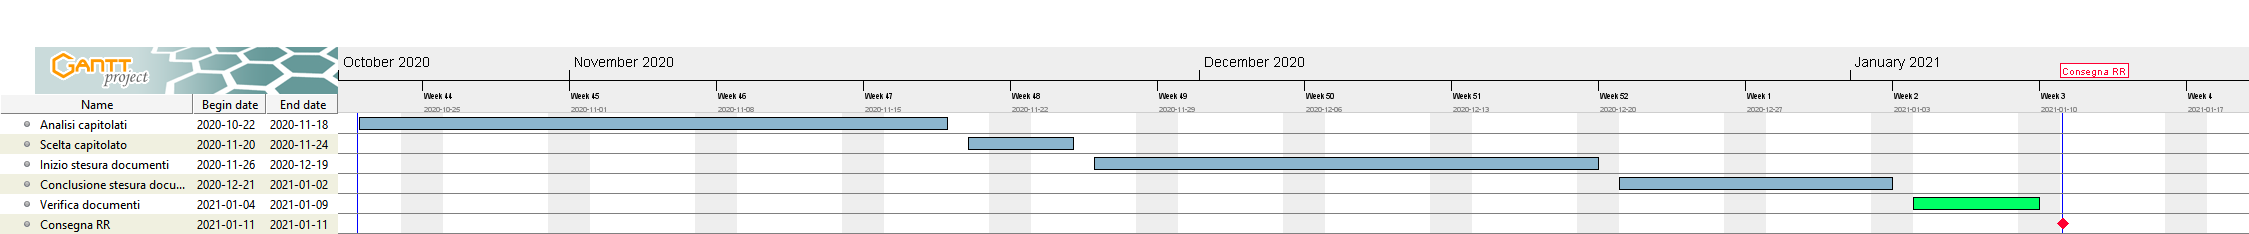
\includegraphics[width=18cm]{img/gantt/01_RR.png}
\caption{ \glossario{Diagramma di Gantt} della fase di analisi dei requisiti}

\end{figure}

\subsection{Consolidamento dei requisiti}%
\label{sub:cons_req}
Periodo: dal 11/01/2021 al 18/01/2021.\\
La fase di consolidamento dei requisiti inizia subito dopo la consegna della \textsc{Revisione dei Requisiti}; prevede l’approfondimento delle tecnologie richieste attraverso lo studio autonomo, l'approfondimento dell'analisi dei requisiti con eventuali aggiornamenti, se necessario. Sarà inoltre previsto qualche contatto con la \emph{Zucchetti S.p.A.} per fugare eventuali dubbi. Per concludere verrà preparata la presentazione. Questa fase si conclude con la presentazione della \textsc{Revisione dei Requisiti} giorno 18/01/2021.

\begin{figure}[H]
\centering
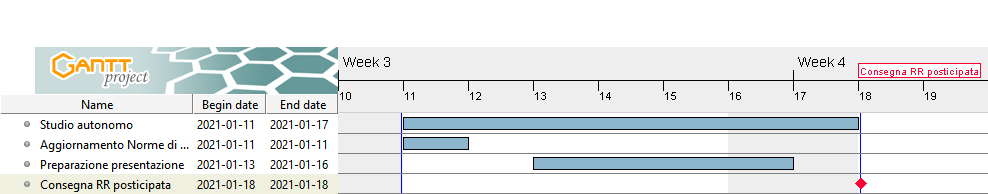
\includegraphics[width=18cm]{img/gantt/01_RR_consolidamento.png}
\caption{ Diagramma di Gantt della fase di consolidamento dei requisiti}
\end{figure}

\subsection{Progettazione architetturale}%
\label{sub:prog_arc}
Periodo: dal 19/01/2021 al 01/03/2021.\\
La fase di progettazione architetturale inizia subito dopo la presentazione della Revisione dei Requisiti.\\
In questa fase verranno aggiornati i documenti redatti, adattati i requisiti in base ai feedback del proponente, verrà fatto uno studio più approfondito delle tecnologie coinvolte, al fine di realizzare un \glossario{Proof of Concept} che farà da base per la fase successiva. Verrà infine scritta la lettera di presentazione al fine di candidarsi alla \textsc{Revisione di Progettazione}. Nella settimana successiva alla consegna della \textsc{Revisione di Progettazione} verrà redatta la presentazione da portare in sede di revisione programmata giorno 08/03/2021. \\ \\

Più in dettaglio, verranno aggiornati i seguenti documenti, portandoli alla versione 2.0.0 in corrispondenza della consegna:

\begin{itemize}
    \item Norme di Progetto;
    \item Glossario;
    \item Analisi dei Requisiti;
    \item Piano di Progetto;
    \item Piano di Qualifica.
\end{itemize}

Verrà anche redatto un nuovo documento chiamato Technology Baseline, che servirà al gruppo per comprendere appieno l'utilizzo di tutte le tecnologie coinvolte per lo sviluppo del prodotto. Verrà scelta un'architettura per il codice identificando il design pattern che meglio si adatta alle nostre esigenze. Verrà sviluppato anche un Proof of Concept che servirà a verificare con il proponente le scelte effettuate per la scrittura del software. Ovviamente, sarà solo un prototipo attraverso il quale si mostreranno solo alcuni dei requisiti obbligatori richiesti, e nemmeno completi. Per le prossime fasi, questo prototipo verrà usato come base e migliorato fino al raggiungimento degli obiettivi prefissati.

Durante la stesura della Technology Baseline sono previsti 2 incrementi:
\begin{itemize}
    \item Incremento 1 (dal 2021-02-11 al 2021-02-20): l'obiettivo principale è la codifica di alcuni requisiti fondamentali concordati con il proponente. Ci si focalizzerà sull'interazione con la libreria D3.js per la creazione dei grafici Scatter Plot Matrix. In particolare sui requisiti: RFO1.2, RFO2.2, RFO3, RFO3.1, RFO3.2, RFO3.3, RFD4.2, RFD4.2.1, RFD4.2.4, RFD4.2.5;
\item Incremento 2 (dal 2021-02-21 al 2021-02-26): l'obiettivo, di questo periodo, sarà l'implementazione dei requisiti incompleti e nel miglioramento generale di tutto il resto. Se i requisiti citati al punto precedente saranno completati, si proverà ad implementare anche alcuni requisiti opzionali come: RFD4.2.2, RFD4.2.3.
\end{itemize}

\begin{figure}[H]
\centering
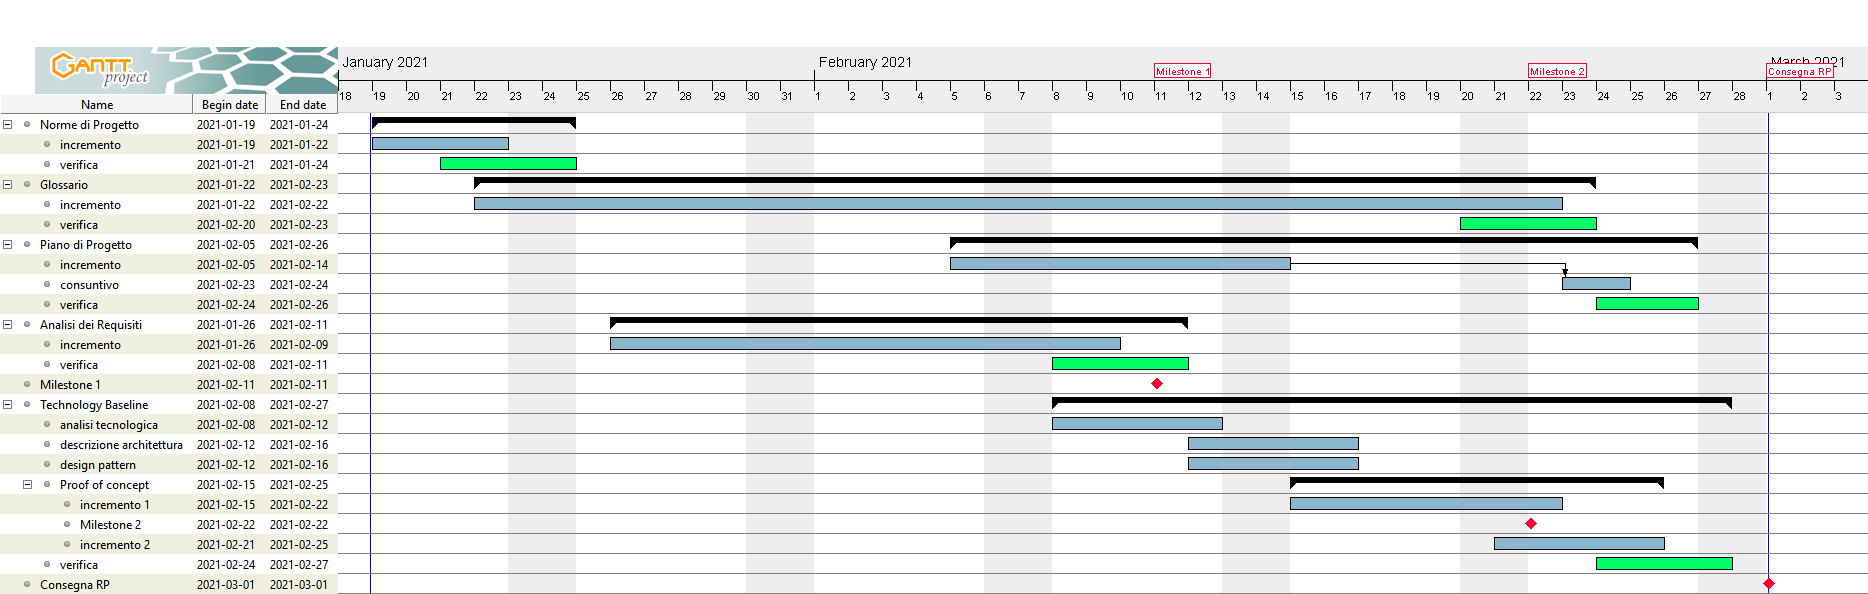
\includegraphics[width=18cm]{img/gantt/02_RP.png}
\caption{Diagramma di Gantt della fase di progettazione architetturale}
\end{figure}

\subsection{Progettazione di dettaglio e codifica}%
\label{sub:prog_dett}
Periodo: dal 01/03/2021 al 02/04/2021.\\
Questa fase prevede la stesura del codice sulla base dei dettagli precedentemente tracciati; vi saranno aggiustamenti della pianificazione e aggiornamenti dei documenti. Verrà inoltre redatto il \textsc{\glossario{Manuale d’utente}}. I contatti con il proponente si manterranno stretti al fine di poter effettuare i primi rilasci e assicurarsi di essere in linea con le richieste.\\
Per concludere verrà redatta la lettera di presentazione per candidarsi alla \textsc{Revisione di Qualifica}. Nella settimana successiva alla consegna della \textsc{Revisione di Qualifica} verrà redatta la presentazione da portare in sede di revisione programmata giorno 09/04/2021. 

\begin{figure}[H]
\centering
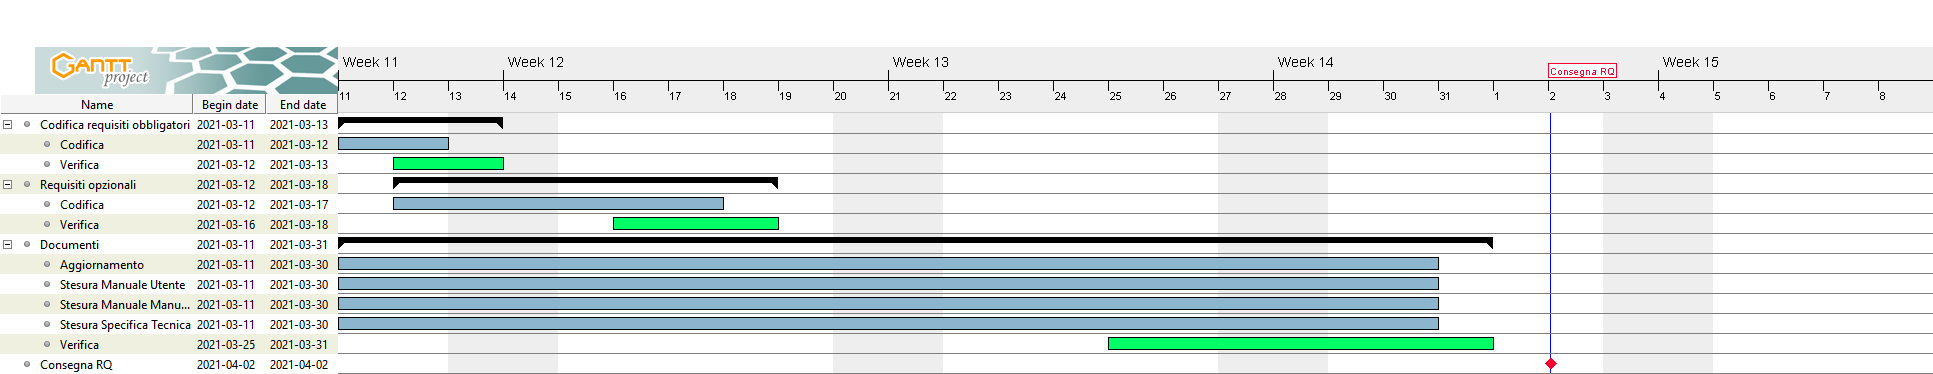
\includegraphics[width=18cm]{img/gantt/03_RQ.png}
\caption{Diagramma di Gantt della fase di dettaglio e codifica}
\end{figure}

\subsection{Validazione e Collaudo}%
\label{sub:valid_coll}
Periodo: 03/04/2021 al 03/05/2021.\\
Questa fase terminerà con la \textsc{Revisione di Accettazione}; in questo periodo verranno aggiornati i documenti e verrà verificato il software creato. Saranno impiegati principalmente verificatori e programmatori al fine di effettuare un controllo serrato sul software che verrà rilasciato. Sarà completato il \textsc{Manuale d'utente} e sarà redatta la presentazione e la lettera finale. Nella settimana successiva alla consegna della \textsc{Revisione di Accettazione} verrà redatta la presentazione da portare in sede di revisione programmata giorno 10/05/2021.

\begin{figure}[H]
\centering
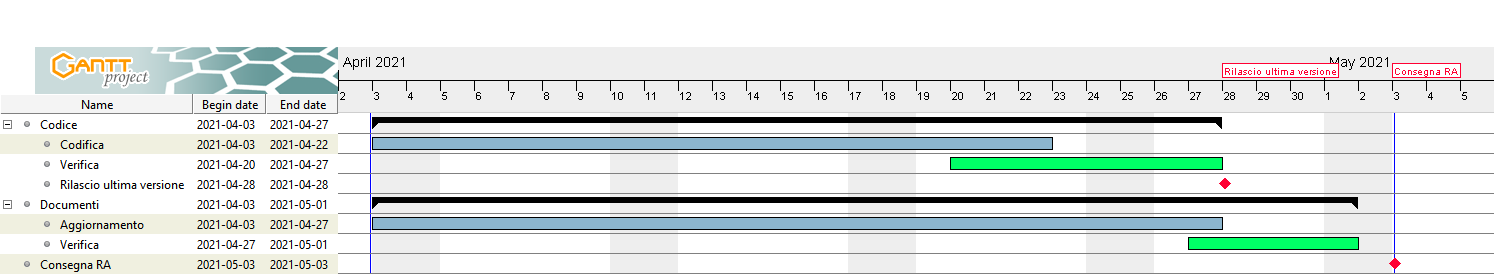
\includegraphics[width=18cm]{img/gantt/04_RA.png}
\caption{Diagramma di Gantt della fase di validazione e collaudo}
\end{figure}

\end{document}